\chapter{Technological Aspects}
To be able to understand the technological aspects of this game and the game's potential, we have to learn more about the technology it will be built upon.  The purpose of this chapter is to get a fundamental understanding of what video games, and in particular exergames, are, and how these type of games are being used today. We will look into different types of technologies related to exergames, as well as examples of exergames used for exercise and rehabilitation. Based on this, we will provide a brief evaluation of Cyberlab's choice of technology and its potential as a tool for exercise and rehabilitation.  \\ \\ 
We will in this section describe different technologies related to video games and exergames. We will also look at related work where the different technologies are tested and evaluated as exercise and rehabilitation tools. Finally, we give our evaluation and recommendation.\\ \\

\section{Computer and Video Games}
"Video games are electronic, interactive games known for their vibrant colors, sound effects, and complex graphics" \cite{videogamedef}. Characters or objects are controlled by hand held game controllers, or by pure body movement captured by sensors or motion controllers. Since the first computer game was developed in 1952 there has been a tremendous evolution in the computer and video game market. Today's market consist of an endless amount of various computer games, video games and video game consoles, and this type of technology is widely used all over the world. It has been developed a game for almost every need and interest, and video games are used for many different purposes, like education and learning, exercising or just pure entertainment. In this section we will describe the history of computer and video games, and gaming statistics. \\ \\
The single-player game, “OXO”, was created in 1952 by A.S Douglas as the first graphical computer game. It was based on a version of Tic-Tac-Toe and designed for academic purposes.  Douglas wrote a PhD degree on Human-Computer interaction, and used feedback from the electronic "OXO" in his work \cite{abouthiginbotham}. Ralph Baer, a German-born television engineer, designed in 1967 a video game console for use on standard television, which was the first of its kind. The game was played by two gamers by connecting two consoles to a television. "Chase" was the name of the game and the purpose was to chase each other by controlling two squares \cite{videogameHistory}. Various features were added to this idea, and this ended up in a series of 12 games known as the Brown Box. Baer introduced his idea to Magnavox, which built apon this Brown Bow prototype. The lead to the release of the Magnavox Odyssey in 1972, which the first commercial video game ever made. However, the Odyssey did not get very popular and faced very low sales numbers. The market for video games experienced huge changes in 1985 when the Nintendo Entertainment System was released. Retailers were sceptic to a new console so soon after the Odyssey failure, but the games Nintendo introduced got popular. Nintendo broke sale records and became the bestselling console at that time \cite{consoleHistory}. \\ \\
The Nintendo Wii is one of many gaming consoles, and it is worldwide very popular. In 2010 it had sold over 30 million units in the US and in Japan there had been sold almost 10 million. These numbers combined with the international market gave Nintendo Wii a total sale of 65.32 million units, see Figure \ref{fig:ConsoleWarWii}. Another gaming console is the Microsoft Xbox 360. Since it was released in 2006 it has experienced strong sales number, and it is today with Nintendo Wii one of the leading gaming consoles on the market. Figure \ref{fig:XboxWiiSales} shows the Xbox 360 and Nintendo Wii's total sale of consoles and games worldwide in 2012. We can see that Xbox 360 and Nintendo Wii have sold the extreme amount of 700 million and 820 million games, respectively. We also observe that Nintendo Wii has sold 97 million units of gaming consoles. However, the bestselling console ever is the Sony PlayStation 2, with over 138 million units sold \cite{statistics2012}. \\ \\

\begin{figure}[h!]
\begin{center}
\includegraphics[scale=0.5]{consolewarwii}
\caption[Nitendo Wii console sale]{Nintendo Wii console sale 2010 \cite{statistics2012}}
\label{fig:ConsoleWarWii}
\end{center}
\end{figure}

\begin{figure}[h!]
\begin{center}
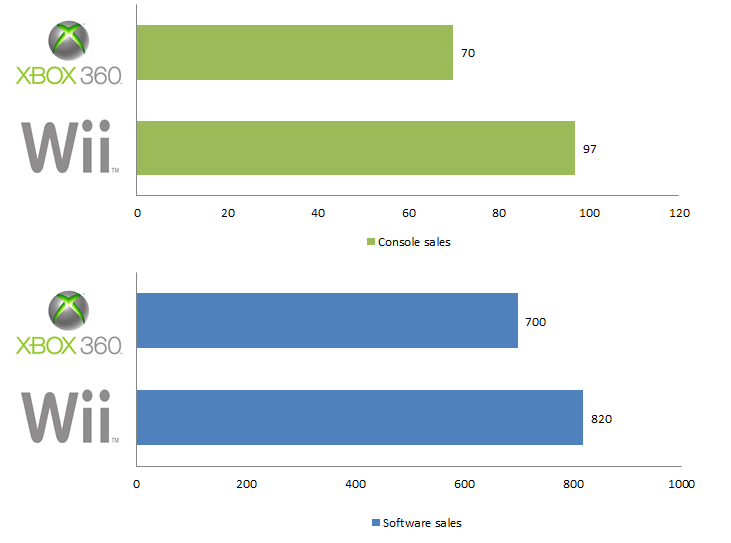
\includegraphics[scale=0.7]{xboxwiisales}
\caption[Nitendo Wii and Xbox 360 sales]{Nintendo Wii and Xbox 360 approximate total console and software sale in 2012 \cite{nintendolife} \cite{microsoftxbox} \cite{vgchartzxbox} \cite{vgchartzwii} \cite{vgchartzhardware}}
\label{fig:XboxWiiSales}
\end{center}
\end{figure}

\begin{figure}
\begin{center}
\includegraphics[scale=0.5]{gamersus}
\caption[Gamer age distribution]{Gamer age distribution in the US in 2010 [modified from \cite{statistics2012}]}
\label{fig:GamersUS}
\end{center}
\end{figure}
DFC Intelligence is a marked research and consulting firm which focus on interactive entertainment and game markets. DFC Intelligence's reports show that the global market for video games experienced a total revenue of 67 billion dollars in 2012. In their new reports they forecast that the global video game market is expected to reach 82 billion dollars in 2017. This number includes revenue from console hardware and software, PC games and games for mobile devices \cite{videogameforcast} \cite{aboutdfcint}.\\ \\
In the last 30 years there has been a great evolution in video games. Video games have become widespread entertainment, and in 2010 as much as 65 percent of all households in the US played video games. The majority of these gamers are in the age of 18-49, and an interesting fact is that there are a greater share of gamers over the age of 50 than there are gamers under 18 \cite{statistics2010} \cite{statistics2012}, see Figure \ref{fig:GamersUS}. Another surprising fact about the gaming statistics in the US is that as much as 47 percent of all gamers are women, see Figure \ref{fig:GenderGamePlayers}, and that there are more female gamers over 18 than male gamers under the age of 17 \cite{statistics2012real}. \\ \\
Video games have become a great part of people's everyday life. It is shown that gamers play about 8 hours a week \cite{statistics2010}. Games that have become very attractive are them involving social interaction. A third of all gamers plays social games and 78 percent are playing with others in-person or online. We can see this from the video game market, as the two best-selling video games in 2011 is Call of Duty: Modern Warfare 3 and Just Dance 3, which both are social games where you have the possibility to play with others \cite{statistics2012real}. \\ \\ 
\begin{figure}
\begin{center}
\includegraphics[scale=0.7]{gendergameplayers}
\caption[Gender of gameplayer]{Video game statistics from 2012 shows that as much as 47 percent of gamers are women \cite{statistics2012real}]}
\label{fig:GenderGamePlayers}
\end{center}
\end{figure}
\begin{figure}
\begin{center}
\includegraphics[scale=0.9]{gamestatisticsnorway}
\caption[Use of computer or video games, Norway, 2011]{Percentage of the Norwegian population that use computer or video games on an average day in 2011, sorted by age \cite{ssb2011}}
\label{fig:GameStatisticsNorway}
\end{center}
\end{figure}
       
"Norsk mediebarometer", a report containing statistics around the topic of media use in Norway, show that 17 percent of the Norwegian population play computer or video games on a normal day in 2011. This includes not only children and teenagers; also a significant share of elderly has started to use computer or video games. 8 percent of the population in the age 45 - 79 years use this kind of technologies on an average day, see Figure \ref{fig:GameStatisticsNorway}, where females are the most active gamers. Norway does not have the same share of elderly gamers as the US, but statistics shows that use of computer and video games in Norway has increased from 5 percent in 2010, and this measurement is the highest share ever recorded \cite{ssb2010} \cite{ssb2011}. One thing worth mentioning about the report of media use in Norway, is that when it came to looking at video games alone, 0 percent of the population in the age 45 - 79 said that they played video games on an average day in 2011. \cite{ssb2011}

\section{Exercise Games}
The new generation of video games combining game play and physical activity is called exercise games, or "exergames". Exergames use technology like motion sensors and remote control to track body movements. This requires the player to get up from the coach and physically move their body to be able to play the game, which stimulates exercise. Exergames are proved to be motivating because it is fun, accessible and easy to understand, and it has shown promise in effecting users health in a positive direction \cite{promotingexercise}. The combination of movement, amusement and social interaction provides exergaming great potential for new business opportunities for the entertainment, recreation and healthcare sectors \cite{gamingforhealth}. Today there exist numerous types of games and technologies related to exergames, where Nintendo Wii, Dance Dance Revolution, PlayStation EyeToy, PlayStation Move and Xbox Kinect are some of the more familiar technologies. \\ \\
Due to the growing interests one has seen it as relevant to study the use of exergames in regard of health and education. The technology these games provide can help improving peoples health in a new and interesting way \cite{gamingforhealth}. In the past years exergames research has increased dramatically, which indicates that it will continue to do so \cite{chamberlin2008exergames}. Research shows tremendous promise in academic and physical progress in youth using exergames. Exergames have also shown an important social aspect, because of the possibility to play with others. This may especially be entertaining for elderly who are often alone and experience loneliness as a part of the everyday life \cite{exergamesforelderly}. \\ \\
The health sector is now more focused on prevention of illness instead of treatment, and research shows that exergames can be used as a tool for this  \cite{gamingforhealth}. Exergames has shown promise for use in rehabilitation, e.g. after stroke or damage to the spine \cite{lange2011development}. Exergames provides users with a feeling of accomplishment by reaching goals, completing exercises and being physically active, which again increases the users mood \cite{staiano2011exergames}. The fun and challenges the game provides could take focus away from boredom and physical pain which makes it appropriate as an exercise or rehabilitation tool \cite{roleofvideogames} \cite{exergamesforelderly}. Games like Wii Sports and Dance Dance Revolution were designed to encourage physical activity, but many other currently available exergames were not designed for this purpose. Few commercial games are suitable for the focused, controlled exercise required for therapy \cite{lange2011development}. Games today are too complicated, go too fast and are too difficult to handle for the elderly. In addition they have too complex and cumbersome consoles \cite{exergamesforelderly}. However, the popularity of exergames and the increasing customer appeal will improve design principles and physical requirements in the future\cite{chamberlin2008exergames}. \\ \\
We will now describe some of the different video game consoles that can be used for exergaming.
\subsection{Dance Dance Revolution}
\ac{ddr} is a series of video games created by Konami Corporation’s Bemani music games division. \ac{ddr} is a rhythmic dance simulation game and was first released as an arcade game in 1998. In few years it became very popular, and the game has had its appearance on several game console systems like Sony PlayStation, Nintendo 64, Microsoft Xbox and Nintendo GameCube \cite{bogost2005rhetoric}. DDR uses a touch-sensitive dance pad with sensors to register movements, where one shall press the right sensors in proper time with electronic dance music. Arrows on the screen give direction on how and when to move around. The DDR games have varying difficulty, requiring different levels of physical activity. GetUpMove.com is an information website about the use of PlayStation Dance Dance Revolution as a weight loss tool. This site was launched in 2004, and one of the highlighted stories was about a young woman who lost about 95 pounds by using DDR. This and similar stories got widespread exposure, and consumers started to buy DDR solely for the purpose of exercise \cite{bogost2005rhetoric}. In 2003, 5 years after the first release, Konami announce that DDR has reached a total sale of 6,5 million units worldwide \cite{gamespot}. 8 years later, in 2011, the number of sold units had reached over 13 million, which are about 1 million units sold every year since the first release in 1998 \cite{gaygamer}. 
\begin{figure}[h!]
\begin{center}
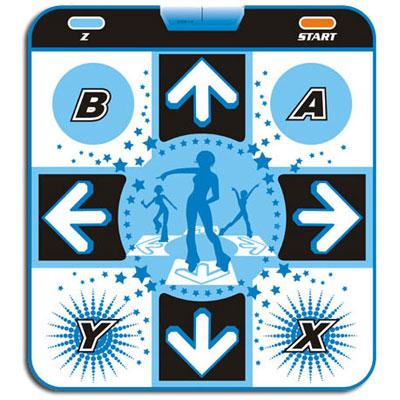
\includegraphics[scale=0.5]{ddrpad}
\caption[Dance Dance Revolution]{The Dance Dance Revolution dance pad}
\label{fig:DDRPad}
\end{center}
\end{figure}

\subsection{PlayStation EyeToy}
In the early 2000s the PlayStation 2 EyeToy was released by Sony Inc. It was the first in this category of games to introduce a device that could translate human motions into a controller input and allow players to physically interact with virtual objects using their own body and without being connected to wires. Human body movements are translated real-time into the controller input by a USB camera  and can also map the player’s face onto in-game characters. Eye Toy is easy to set up and its applications offer a lot of different environment and can be played by one or more players. \cite{eyetoy}
\begin{figure}[h!]
\begin{center}
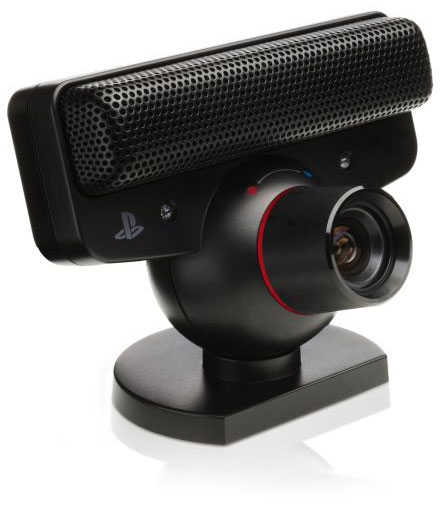
\includegraphics[scale=0.3]{pseyetoy}
\caption[PlayStation EyeToy]{The PlayStation EyeToy}
\label{fig:PSEyetoy}
\end{center}
\end{figure}
\subsection{PlayStation Move}
PlayStation Move was released in September 2010. The PlayStation Move’s interface consists of the Move Eye, a RGB camera with directive microphones, and the Motion Controller, a wand with an illuminating sphere attached to it. The camera can detect the sphere and determine where the wand is, which allows the players to interact with the game through motion and position. The sphere attached to the wand helps the camera to determine the distance from the wand to the camera and to track the controller's position in three dimensions. The wand is equipped with a three-axis accelerometer and a three-axis gyro sensor which is used to track rotation in overall motion and can also be used to detect if the wand is out of range (i.e. hidden behind the player back). \cite{comparison} Up to four wands are supported at one time, which makes it possible for four players to play together. The color of the sphere can be changed to any color and is usually used to show which player is active and to give visual feedback \cite{ppmove}. The SDK is not made public, so it is difficult for a third party to make original applications \cite{comparison}. 
\begin{figure}[h!]
\begin{center}
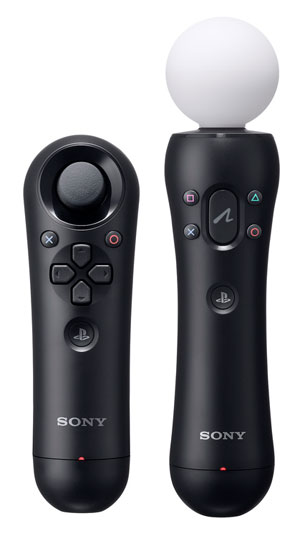
\includegraphics[scale=0.3]{PSmove}
\caption[PlayStation Move]{The PlayStation Move}
\label{fig:PSMove}
\end{center}
\end{figure}

\subsection{Nintendo Wii}
Nintendo Wii was released in 2006 as the first motion sensor game. Only one year and 20 million units sold later, it became the market leader of that times generation of consoles. It consists of a Wii remote, which is the primary controller and a secondary controller called Nunchuk. The Nunchuk is connected at the bottom of the Wii remote control \cite{hackingwii}. The Wii remote contains 12 buttons, a 3-axis accelerometer, a high-resolution highspeed IR camera, a speaker, a vibration motor, and wireless Bluetooth connectivity.
The IR camera is placed on the remote's tip and can track up to four simultaneous IR light with high resolution and high speed. The accelerometer within the remote control provides the Wii remote’s motion-sensing capability. The 12 buttons on the remote are arranged symmetric so that both hands can be utilized. A vibrator motor, LED lights and a small speaker are used for different kinds of user feedback, like varying light strength and sound-effects. The four LED lights are also used to indicate the different players' ID. Communication is sent over the wireless Bluetooth connections, which enables up to four controllers to be connected at the same time.  The users of Nintendo Wii can make their own personal profile, called Mii, where the data of the player will be directly connected up on the remote used  \cite{hackingwii} \cite{whatiswii}. By November 2012 over 97 million Wii consoles were sold \cite{vgchartzhardware}.  To complete the original system with improved accuracy and response time, Nintendo made an enhanced version, Wii Motion Plus, which was released in November 2009 \cite{consoles}. There are several SDKs for Nintendo Wii open, which makes it possible for a third party to develop applications which utilize the controller \cite{comparison}. 
\begin{figure}[h!]
\begin{center}
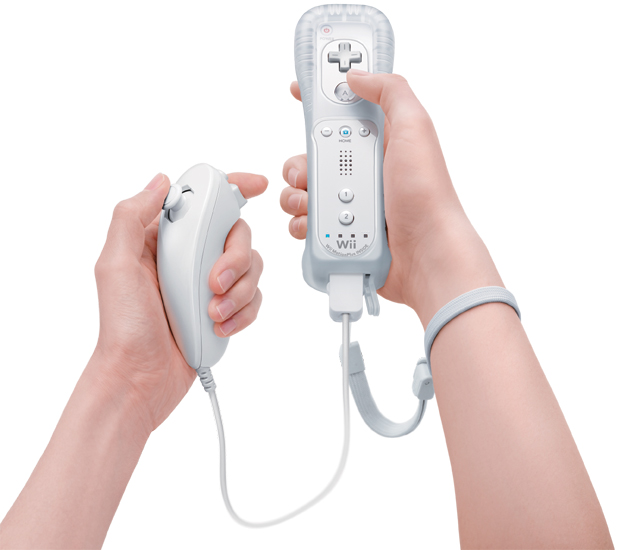
\includegraphics[scale=0.3]{nintendowii}
\caption[Nitendo Wii]{The Nintendo Wii}
\label{fig:NintendoWii}
\end{center}
\end{figure}

\subsection{Wii Fit Plus}
Wii Fit Plus is a video game created for the Wii console. One of its main add-on accessories is the Wii Balance Board. The board can read the players' body movements and give them back on the screen as they are playing, by the use of multiple pressure sensors contained in the board \cite{whatiswiifit}. The board has an area of 55,1 cm {*} 31,6 cm. A third party can also build applications for the balance board using the SDK WiimoteLib \cite{comparison}. It has been shown that game-based balance programs like Wii Balance Board compared to traditional training is easier, more motivating and more enjoyable \cite{taylor2011activity}.
\begin{figure}[h!]
\begin{center}
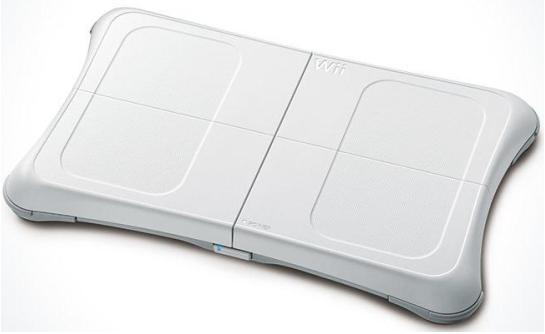
\includegraphics[scale=0.4]{wiibalance}
\caption[Wii Balance Board]{The Wii Balance Board}
\label{fig:WiiBalanceBoard}
\end{center}
\end{figure}

\subsection{Microsoft Kinect for Xbox 360 and Windows}
Microsoft Kinect was released in 2010 and became quickly extremely popular. Only 25 days after its release it had sold 2.5 million units and by January 2012 Xbox 360 had sold over 66 million consoles and more than 18 million Kinect motion sensors \cite{consoles} \cite{kinectsold}. Kinect is a flexible low-cost motion sensor that can track human motions and it can be used with the Xbox 360 game console or with a Windows machine.  The sensor is webcam-based, which enables the user to play and interact with the game without physically holding a sensor device. Instead the player can interact with the game console through a natural user interface by moving their body and by using voice commands. The device has the ability to give full-body 3D motion capture capabilities and gesture recognition by help of its RGB camera and a depth sensor \cite{kinect}. One advantage with Kinect is that it has an interface that senses players various motions and it also senses other objects in the field, which makes a natural environment where the players can interact with virtual objects in the real world. \cite{comparison}. The Kinect sensor for Windows is designed to operate on computers running Windows 7, Windows 8, Windows Embedded Standard 7, and Windows Embedded POSReady 7. All the users need is the Kinect sensor, a computer and a Kinect for Windows application. Kinect for Windows SDK was released in June 2011 and enables developers to build Kinect applications with C++, C\# or Visual Basic using Microsoft Visual Studio 2010. This enables any third party to develop Kinect for Windows applications. \cite{kinectwindows}.\\ \\
\begin{figure}[h!]
\begin{center}
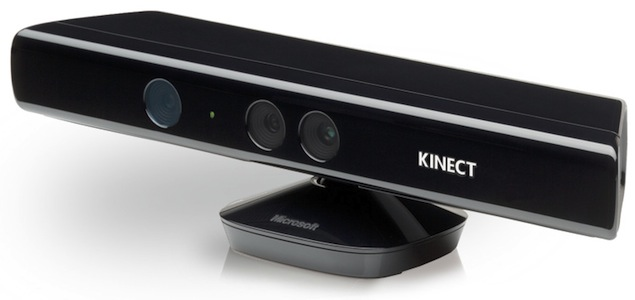
\includegraphics[scale=0.3]{kinect}
\caption[Kinect Sensor]{The Microsoft Kinect Sensor}
\label{fig:KinectSensor}
\end{center}
\end{figure}

\section{Using Video Games for Exercising and Rehabilitation: A background Study}
There have been done several researches on the use of video games for health-related purposes like exercise and rehabilitation. The main focus in these studies are on the physical, social, and cognitive benefits an exergame can provide. We will review the interesting findings we did with emphasis on positive health effect, both physically and psychologically. Studies show that use of video games also has social benefits, which are an important aspect for elderly. This is a group of people that may not have much social interaction, because they are afraid of leaving the house. Providing social interaction through use of exergames can increase quality of life. The research review provided will relate to the already described technologies. Based on the research done we will also include our opinion and evaluation of how suitable exergames are for elderly. \\ \\
Primack et al. \cite{roleofvideogames} did a broad study of video games in the context of improving health, where they analysed 1452 articles with the topic of video games.  For articles to be included in the study, they had to meet criteria for inclusion. Some of the criteria include: involving use of video games, showing health-promoting, clinically relevant outcomes, and being a randomized controlled trial. 38 articles met these criteria and were therefore included in the study. Studies were also considered a "health-promoting, clinically relevant health consequence" if they showed effect on health care providers to improve their patients' health. Based on the purpose of the video game, each of the 38 articles was assigned to one of six categories of improvement; physical therapy, psychological therapy, health education, disease self-management, distract from discomfort, and increase of physical activity. In all of the categories, beside the category of self-management, 67 - 100 percent of the studies showed positive outcomes with the use of video games. The study with the best outcome was distraction from discomfort, where all of the outcomes showed positive effect. However, the results of these studies showed that the most common positive outcome was related to physical therapy, in e.g. rehabilitation after a stroke, and psychological therapy, in e.g. reducing post-trauma. The purpose of this study was to look into the ability of video games to address a variety of health conditions, and results showed that video games can have a positive effect in a variety of categories in all age groups. Video games has also showed positive outcomes when it comes to health-care personnel using this type of technology to train patients. Video games for elderly, individuals in the age group 50 - 80, often focus on age-related changes like decrease of balance and cognitive decline. However, the study showed that the age group with the best opportunity to improve health is in the age group of 30 - 50. The fact that video games show potential health-related benefits is an important finding, as it represents a huge industry for the entertainment sector and as the use of video games has become very popular among people of all ages \cite{roleofvideogames}. \\ \\
Taylor et al. \cite{taylor2011activity} did a review on different studies related to gaming systems in exercise and rehabilitation. We will summarize some of their interesting findings here. From studies that was performed on adolescents and young adults, they found a trend; the  \ac{ee} while playing Wii was greater than when doing sedentary activities, but not greater than brisk walking. This suggests that playing Wii sports could not replace real sports activities. Playing \ac{ddr} on the other hand, maximum heart rate and oxygen consumption were greater compared with Wii sports, suggesting that DDR can substitute physical activity, based on \ac{ascm} guidelines for physical activity. In their research they also found a study on what attitudes people have against \ac{ddr} to encourage exercise. 40 postmenstrual women, aged 45-75 years old were asked. The overall attitude was positive; the game was fun and it gave potential to improve coordination. However, they also expressed a concern about a long learning process. It was also found that playing against a human gave greater arousal ratings and physiological responses to gaming than when playing against a computer, which benefit the enjoyment. This aspect is important to take into consideration when setting up a gaming environment for the older population, because they may benefit from the social interaction. Some games have already shown the potential for rehabilitation, like the EyeToy and the Wii. The main reasons why these type of games a suitable are that they have the ability to increase motivation and produce distraction from daily, boring and painful treatments. Wii is seen as an attractive game for rehabilitation, both at home or in institutions. Wii is actually already in use within the National Health Service in UK and is commonly used for the elderly and patients with pathologies  \cite{taylor2011activity}. \\ \\
Another finding of Taylor et al. was a study done to find out what attitude non-disabled elderly (70 +/- 5,7 years) had to the EyeToy. They were positive: they enjoyed it and found it easy to use. For patients with stroke it appeared to be less suitable, which could be even worse if they had to hold on to a controller, for example with Wii. This suggests that EyeToy is more suitable for patients with stroke than games with remote controllers.  
Even though these type of games are initially meant as entertainment systems, there are a number of studies that have used the hardware and developed software to turn for example the Wii into a useful rehabilitation tool. The importance of these games is entertainment that motivates for actual sports. This is very important in for example rehabilitation \cite{taylor2011activity}. \\ \\
Staiano and Calvert write about the increasing use of exergames in the health sector. Gaming consoles are already integrated into equipment at gyms and health clubs. An example is Concept 2’s rowing machine. Here the people exercising are motivated through competition and through virtual trainers who monitor their progress and encouraging them to proceed to the next level. Feedback from a virtual trainer is also offered in Wii Fit. Also some schools are starting to integrate games into their curriculum. In all of West Virginia’s 765 public schools they have integrated DDR in their physical education. This has proven to be very effective and popular and some students lost 5-10 pounds after playing DDR daily \cite{staiano2011exergames}. \\ \\
Brox et al. \cite{exergamesforelderly} provide a review on how exergames can be used in the elderly populations and specific challenges related to this. In addition to physical challenges related to the older population, there are also cognitive and  mental challenges, like slower information processing, depression and loneliness. Particularly the research team  looked into studies with elderly using Nintendo Wii. Several games have been tested and bowling appeared to be the most suitable game for the older population. One of the main reasons for this is that the participants can take the time they need to throw the ball. Many games appeared to be difficult, but at the same time they gave positive social effect. Also in this paper, it is emphasised that these kind of games are not designed for elderly, where one of the main problem is that the games are found to be too fast. In addition the balance board contained in Wii Fit, may increase the risk of falling during the session. This suggest that other games like  for example EyeToy can  be more suitable, because of the ease of use. They suggest that persuasive technologies should be used to encourage elderly to exercise and they propose some persuasive strategies that can be used for motivation. First, it is important to not show too much  detailed information . The information can rather be showed visual, like for example with a fish that becomes larger and healthier when the participant is exercising. Second, feedback provided during the session should be positive and delivered when the players achieve their goal. However it should not disturb the player with information at inappropriate time. Third, information about past workout sessions should be  provided to help the players set goals for the next session. And finally, the interface of the game should be user friendly and easy to use, so that the user can focus on the exercise and not so much on understanding how to manage the system.  The writers of this paper believe in the use of  exergames as an exercise tool for elderly because of its fun and motivating nature. However, elderly they had talked to expressed that they were afraid that this game would replace ordinary physical treatment. Therefore, they suggest that exergames can be used in addition to regular training, and also as a supplement in training groups, so people can play together. They stress that the social factors are very important  both because of this group often are lonely and also because people get more involved in the activities when participating with others. The conclusion of this article is that to motivate elderly to exercise more, social interactions and exergames should be combined.\cite{exergamesforelderly} \\ \\
Williams et al. \cite{excell} did a study to see if exergames, more specifically Nintendo Wii Fit, was an applicable type of exercise to reduce the falling statistics of community-dwelling people over 70 years. A group who attended Wii Fit exercise sessions was compared with a group who went to a local falls group. 77 percent of the participants said that if the exercise program was more available, people like themselves would use it. 92 percent of the participants expressed that they wanted to exercise with the Wii Fit in the future, while 61 percent would choose to exercise with the Wii Fit rather than attend a falls group. An improvement in \ac{bbs}\footnote{Berg Balance Scale (BBS): This is a performance based measure using 14 activities of daily living (range 0-56)\cite{excell}} after 4 weeks was seen in the group that played Wii Fit, meaning that there is a potential to improve balance in this population. Despite this, there was no change in \ac{fesi}\footnote{The Falls Efficacy Scale - International (FES-I). This scale measures confidence in performing a range of activities of daily living without falling \cite{fes}} after 4 weeks. The qualitative data for the group that played Wii Fit showed improved confidence for the participants. The conclusion of the study was that Wii Fit is acceptable in  older people with a history of falls and that it has the potential to improve balance and confidence. Further work has to be done to find and develop an acceptable exercise program with the potential to improve balance in older individuals \cite{excell}.\\ \\
Chang et al. \cite{kinect} did a study where they prototyped a Kinect game that was designed to help motivate people with motor disabilities to do their exercise more frequently and to improve the motor proficiency and quality of life. Because of the inconvenience of having to wear sensors in some of the other relevant technologies, Chang et al. chose to use Kinect. They developed a game, called "Kinerehab", that was meant to assist therapists in rehabilitating students in public school settings. To detect the students’ movements Kinerehab used image processing technology of Kinect. To engage and motivate the student for physical rehabilitation, the system was made with an interactive interface that had both audio and video feedback. For making it easy for therapists to review the progress of each student quickly, the system also included details of students rehabilitation conditions which was automatically recorded in the system. Two students, a 16 year old girl diagnosed with  muscle atrophy and insufficient muscle endurance, and a 17 year old boy diagnosed with cerebral palsy, were chosen to participate in the study. The girl used a wheelchair and could only stand with assistance. The study included two phases: a baseline phase  where no assistive technology was applied and the intervention phase where the Kinerehab was used. Both phases were done twice, beginning with the baseline phase, continuing with the intervention phase and so on. In both phases the same exercises were done. The result showed that both participants increased the number of correct movements significantly in the intervention phase. On average the number of correct movements was 49 in the first baseline phase (5 sessions), while 170 in the first intervention phase (11 sessions). Both students indicated that the game motivated them to do the exercises and that they wanted to continue using it. The therapists said it would reduce their workload a lot. This suggests that Kinect can be a viable rehabilitation tool, but further work, where more people with disabilities participate, should be done \cite{kinect}. \\ \\ 
Garcia et al. \cite{garcia2012exergames} has developed a game-based exercise on a Microsoft Kinect platform, where the game has stepping exercises specially designed for elderly. The purpose of the Kinect-based exergame was to increase physical strength and improve balance. In the context of developing this game Garcia et al did a review of existing performance-based tests for prevention of fall in older people. They wanted to find a method they could use to see how well their Kinect-based exergame was suited for clinical purposes. They decided to use a \ac{csrt} task, a method used to identify parameters to say something about fall risk.  The Kinect-based game was built upon this \ac{csrt} task, due to its ability to measure parameters with the Kinect, and that it easily could translate into a video game. The Kinect-based game involved a user standing in front of a screen. The body was recognized by the Kinect sensor and an avatar was displayed on the screen.  The avatar was surrounded by sectors which would light up randomly, indicating that the user should step on it. This exercise was based on the original CSRT task, and the purpose was to identify the user’s step length and fall risk. The system could also challenge the user’s cognitive skills by portraying the user from several camera angles, which made the test suitable for calculate cognitive conditions.  The first draft of the game was meant to be controlled in a clinical setting with physiotherapists or other medical personnel. Based on the CSRT task, they included several measurements in their Kinect-based game like movement time and response time. They also added some additional features like validation of direction and step length.  Microsoft Kinect was chosen as platform because of the possibility to capture movement without the use of gaming consoles or wearable sensors. Kinect makes is possible to give full focus to the exercise, and not think about handling different consoles. This makes the game easy to use, as it gives elderly the opportunity to have full focus on the exercise. By freeing their hands they can lower the impact of damage if they were to fall during the exercise. Kinect was also chosen because of the motion capture technology it provides, which makes it possible to test motor and cognitive skills. This is done by providing real-time information about of the body position. The Kinect technology makes it possible measure parameters that can be used as clinical data, which makes it appropriate to use in clinical practice \cite{garcia2012exergames}.\\ \\
We can conclude that there is a lot of attention on the use of video games as an exercise and rehabilitation tool, both for the young, and older population. Exergames have been shown effective and motivating in rehabilitation for young people with disabilities. In this assignment we focus on elderly, but we found it interesting, because we believe that  this type of rehabilitation can also be viable for elderly with the same type of disabilities. An important advantage of using games for rehabilitation is that it distracts the participant from discomfort and pain and reduce post-trauma. In addition it can serve as a more fun and motivating way to exercise. Elderly that participated in one of the studies had positive attitude about the use of a game for exercise, and expressed that they wanted to use it in the future if it was more available. Bringing this game into physical therapy sessions and training groups, will make the game more available, given that the  person attend this kind of meetings. Another arena for this game can be to provide it in their home, making it even more available. However, as mentioned in the previous chapter, we do not think this is the right arena yet.  Some participants  expressed some concern about the learning process. These concerns probably arise from the lack of experience with this kind of technology.  The games are primarily been made for fun and entertainment and are not designed specifically for rehabilitation.  The commercial games offered today are too rapid and too complicated for the older population. Older people often face challenges like slower information processing and learning. It is therefore a need for customized games for this group. The game should be easy to understand and give feedback in a way that is informative but not disturbing. Other important finding is that arousal ratings was greater when playing against a human rather than playing against a machine and that the social factors of playing a game are important. This suggests that the exergame should have the ability for multiplay.  \\ \\
Based on the study we did on the different technologies available and research done by others, we conclude that the Kinect sensor is a viable choice of technology for the development of an exergame for elderly. The main reason is the convenience of not having to hold on to a device. Nintendo Wii has been tested as a rehabilitation tool, and has in some cases shown to be effective. However, the use of a controller and a balance board complicates the game and can heighten the threshold to use the game. It can also contribute to increasing the risk of falling.  Use of a technology where only body movements can be used to control the game, will be more convenient for the older population. In addition, the Kinect sensor has proved to accurately measure body movements and that the parameters retrieved from the sensor can be used for clinical practice which is important when using the game for rehabilitation. Finally,  it is easy to develop a game for this platform, enabled by the free SDK offered.\\ \\





